\section{Results}

\subsection{Simulator Evaluation}

\begin{slide}

    \inote{
        \item TODO: Talk about the overhead
    }
\end{slide}

\subsection{Cooperativity Mechanics}


\begin{slide}
    Longevity-Based Batching Scheduler:
    \begin{itemize}
    \item Spawn Mechanism 
    \item[] ~~~~{\it (Where does a new process go if batch is too big?)}
    \end{itemize}
    
    Channel Pinning Scheduler:
    \begin{itemize}
    \item Channel Spread 
    \item[] ~~~~{\it (How to spread the channels across processors?)}
    \end{itemize}

    Bipartite-Graph Aided Sorting Scheduler:
    \begin{itemize}
    \item Channel Implementation 
    \item[] ~~~~{\it (Does blocking help to take advantage of sorting?)}
    \end{itemize}

    \inote{
        \item LBB: Can also look at how the batch size effects different types
            of behaviours.
        \item SS: Could also look at a stealing mechanism.
    }
\end{slide}

\begin{slide}
\framesubtitle{Longevity-Based Batching Scheduler}

        \begin{table}[htp!]
            \centering
            \begin{tabular}{@{}cccc}
                & \multicolumn{3}{c}{$PRing_N$} \\ \cline{2-4}
            & $N=P=8$ & $N=B=10$ & $N=2*B=20$     \\ \cline{2-4} 
                \multicolumn{1}{c|}{\rotatebox{90}{\rlap{\textbf{Reduc. Density}}}} & 
            \multicolumn{1}{c|}{\includegraphics[scale=0.15]{tests/pring/longbatcher/8/pg_0004.pdf}} & 
            \multicolumn{1}{c|}{\includegraphics[scale=0.15]{tests/pring/longbatcher/10/pg_0004.pdf}} & 
            \multicolumn{1}{c|}{\includegraphics[scale=0.15]{tests/pring/longbatcher/20/pg_0004.pdf}} \\ 
            \cline{2-4} 
        \end{tabular}
        \caption{Comparison of different sized $PRing_N$ on the Longevity 
                 Batching Scheduler with batch size $B=10$.}
            \label{tab:pring-longbatcher-testing}
        \end{table}

    \inote{
        \item Before talking about spawn mechanism, pointing out the
              primary goal and effect of batching to catch the granularity
              of the application.
    }
\end{slide}
\begin{slide}
\framesubtitle{Longevity-Based Batching Scheduler}
    \inote{
        \item TODO: Get simple $ClusterComm_{(N,1)}$ or the PTree results to contrast with PRING 
        \item This brings it back to an issue of behaviour recognition.
    }
\end{slide}


\begin{slide}
\framesubtitle{Channel Pinning Scheduler}
    \begin{table}
    \centering
    \begin{tabular}{@{}ccc}
    & \multicolumn{2}{c}{$Interactivity_{(20,0)}$} \\ \cline{2-3} 
    & \multicolumn{1}{c}{$MTRRWS$-$SQ$}       & \multicolumn{1}{c}{Channel Pinning} \\ \cline{2-3} 
 
    \multicolumn{1}{c|}{\rotatebox{90}{\rlap{~~Queue Length}}} &
    \multicolumn{1}{c}{\includegraphics[scale=0.15]{tests/interactivity/20/wssq/ca/pg_0003.pdf}} & 
    \multicolumn{1}{c|}{\includegraphics[scale=0.15]{tests/interactivity/20/cp/ca/pg_0003.pdf}} \\

    \multicolumn{1}{c|}{\rotatebox{90}{\rlap{Reduc. Density}}} &
    \multicolumn{1}{c}{\includegraphics[scale=0.15]{tests/interactivity/20/wssq/ca/pg_0004.pdf}} & 
    \multicolumn{1}{c|}{\includegraphics[scale=0.15]{tests/interactivity/20/cp/ca/pg_0004.pdf}} \\ \cline{2-3}
    \end{tabular}
    \label{tab:cp-compare-rand-uniform-ca}
    \end{table}

    \inote{
        \item Comparison of Uniform synchronization for $MTRRWS$-$SQ$ 
                and the Channel Pinning Scheduler on Absorption Channels.
        \item This used the $even$ spread type.
        \item Note the speed at which it saturates all cores.
        \item Despite Naive WS, we still have decent spread.
    }
\end{slide}

\begin{slide}
\framesubtitle{Bipartite-Aided Graph Sorting Scheduler}

    \begin{table}
    \centering
    \begin{tabular}{@{}ccc}
        & \multicolumn{2}{c}{Parallel Fibonacci} \\ \cline{2-3}
        & $MTRRWS$-$SQ$ & Sorting Scheduler  \\ \cline{2-3} 
        \multicolumn{1}{c|}{~}  & 
        \multicolumn{1}{c|}{\includegraphics[scale=0.27]{tests/pfib/wssq/pg_0001.pdf}} & 
        \multicolumn{1}{c|}{\includegraphics[scale=0.27]{tests/pfib/ss/pg_0001.pdf}} \\ \cline{2-3}
    \end{tabular}
    \label{tab:ss-compare-fib}
    \end{table}

    \inote{
        \item Channel State comparison of Parallel Fibonacci executed on 
                $MTRRWS$-$SQ$ and the Bipartite-Graph Aided Sorting Scheduler. 
        \item Note the large reduction in number of ticks.
    }
\end{slide}

